\documentclass{article}
\usepackage{amsmath}
\usepackage{amssymb}
\usepackage{graphicx}
\usepackage{hyperref}
\usepackage[version=4]{mhchem}

\title{Example 7}
\date{}

\begin{document}
\maketitle

Let \(r_{1}, r_{2}\), and \(r\) be the radii of three circles as shown in the figure.\\
Show that \(\frac{1}{\sqrt{r}}=\frac{1}{\sqrt{r_{1}}}+\frac{1}{\sqrt{r_{2}}}\).

Proof:
\begin{center}
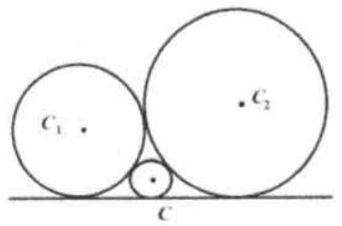
\includegraphics[width=\textwidth]{images/problem_image_1.jpg}
\end{center}

Applying Pythagorean Theorem three times:\\
\(M N=\sqrt{\left(r_{1}+r\right)^{2}-\left(r_{1}-r\right)^{2}}=2 \sqrt{r_{1} r}\)\\
\(N P=2 \sqrt{r_{2} r}\)\\
\(M P=2 \sqrt{r_{2} r_{1}}\).\\
We see that \(\sqrt{r_{1} r}+\sqrt{r_{2} r}=\sqrt{r_{1} r_{2}}\).\\
\centering
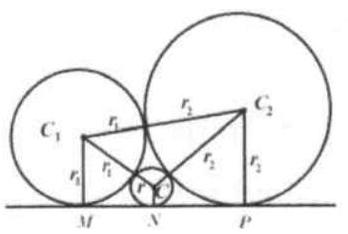
\includegraphics[width=\textwidth]{images/reasoning_image_1.jpg}\\
\(\Rightarrow \quad \frac{1}{\sqrt{r}}=\frac{1}{\sqrt{r_{1}}}+\frac{1}{\sqrt{r_{2}}}\).


\end{document}
